\documentclass[12pt]{article}

\usepackage{cite}
\usepackage[colorlinks,
linkcolor=blue,
anchorcolor=black,
citecolor=black]{hyperref}
\date{}
\usepackage{hyperref}
\usepackage{graphicx} 
\usepackage{float}
\usepackage{subfigure}
\usepackage{geometry}
\geometry{letterpaper,left=3cm,right=3cm,top=2cm,bottom=3cm}
\title{U-Net Based Brain Segmentation}
\author{Yanlong Sun}
\begin{document}
\maketitle
 \urldef{\myurl}\url{https://github.com/yanlong-sun/brain_segmentation.git}

\begin{abstract}
MRI can provide important information for surgeon before the surgery and provide researchers more immediate information to study the organ structure. However, manually extracting is always costly. This experiment utilized a deep learning model to segment the brain automatically and achieved a great performance.
\end{abstract}

\section{Introduction}
In this experiment, we replicated a deep learning model with the U-Net architecture \cite{buda} to segment the brain MRI. After simply amended the input and output, we can easily utilize this model to segment brain MRI in different size with a high accuracy.  The codes are available at the following link: \myurl
\section{Method}

\subsection{Preprocessing}
The image data we used in this experiment for training is Calgary-Campinas-359 \cite{dataset}(CC-359) dataset. In order to improve the contrast for some low contrast slices and keep all slices have similar contrast, we used histogram equalization to process MRI slices. Besides, all of the slices are supposed to have the same and specific size to be input into the neural network. So we cut the edges or padded zeros to slices. In a nutshell, the preprocessing of the MRI subjects includes the following steps:
\begin{itemize}
	\item Use histogram equalization to increase the global contrast of the images 
	\item Pad zeros to the slices and masks at the same time according to their aspect ratio.
	\item Center crop the slices and masks into size of 256*256.
\end{itemize} 



\subsection{Segmentation}
We kept the structure of the original model but retrained the model. After training on preprocessed CC0001-CC0030 of CC-359, about 7000 slices, we got the Average Dice coefficient of 92.13\% on 18 test subjects. Figure 1 shows our segmentation results of 3 subjects.
\begin{figure}[H]
\centering 
\subfigure{
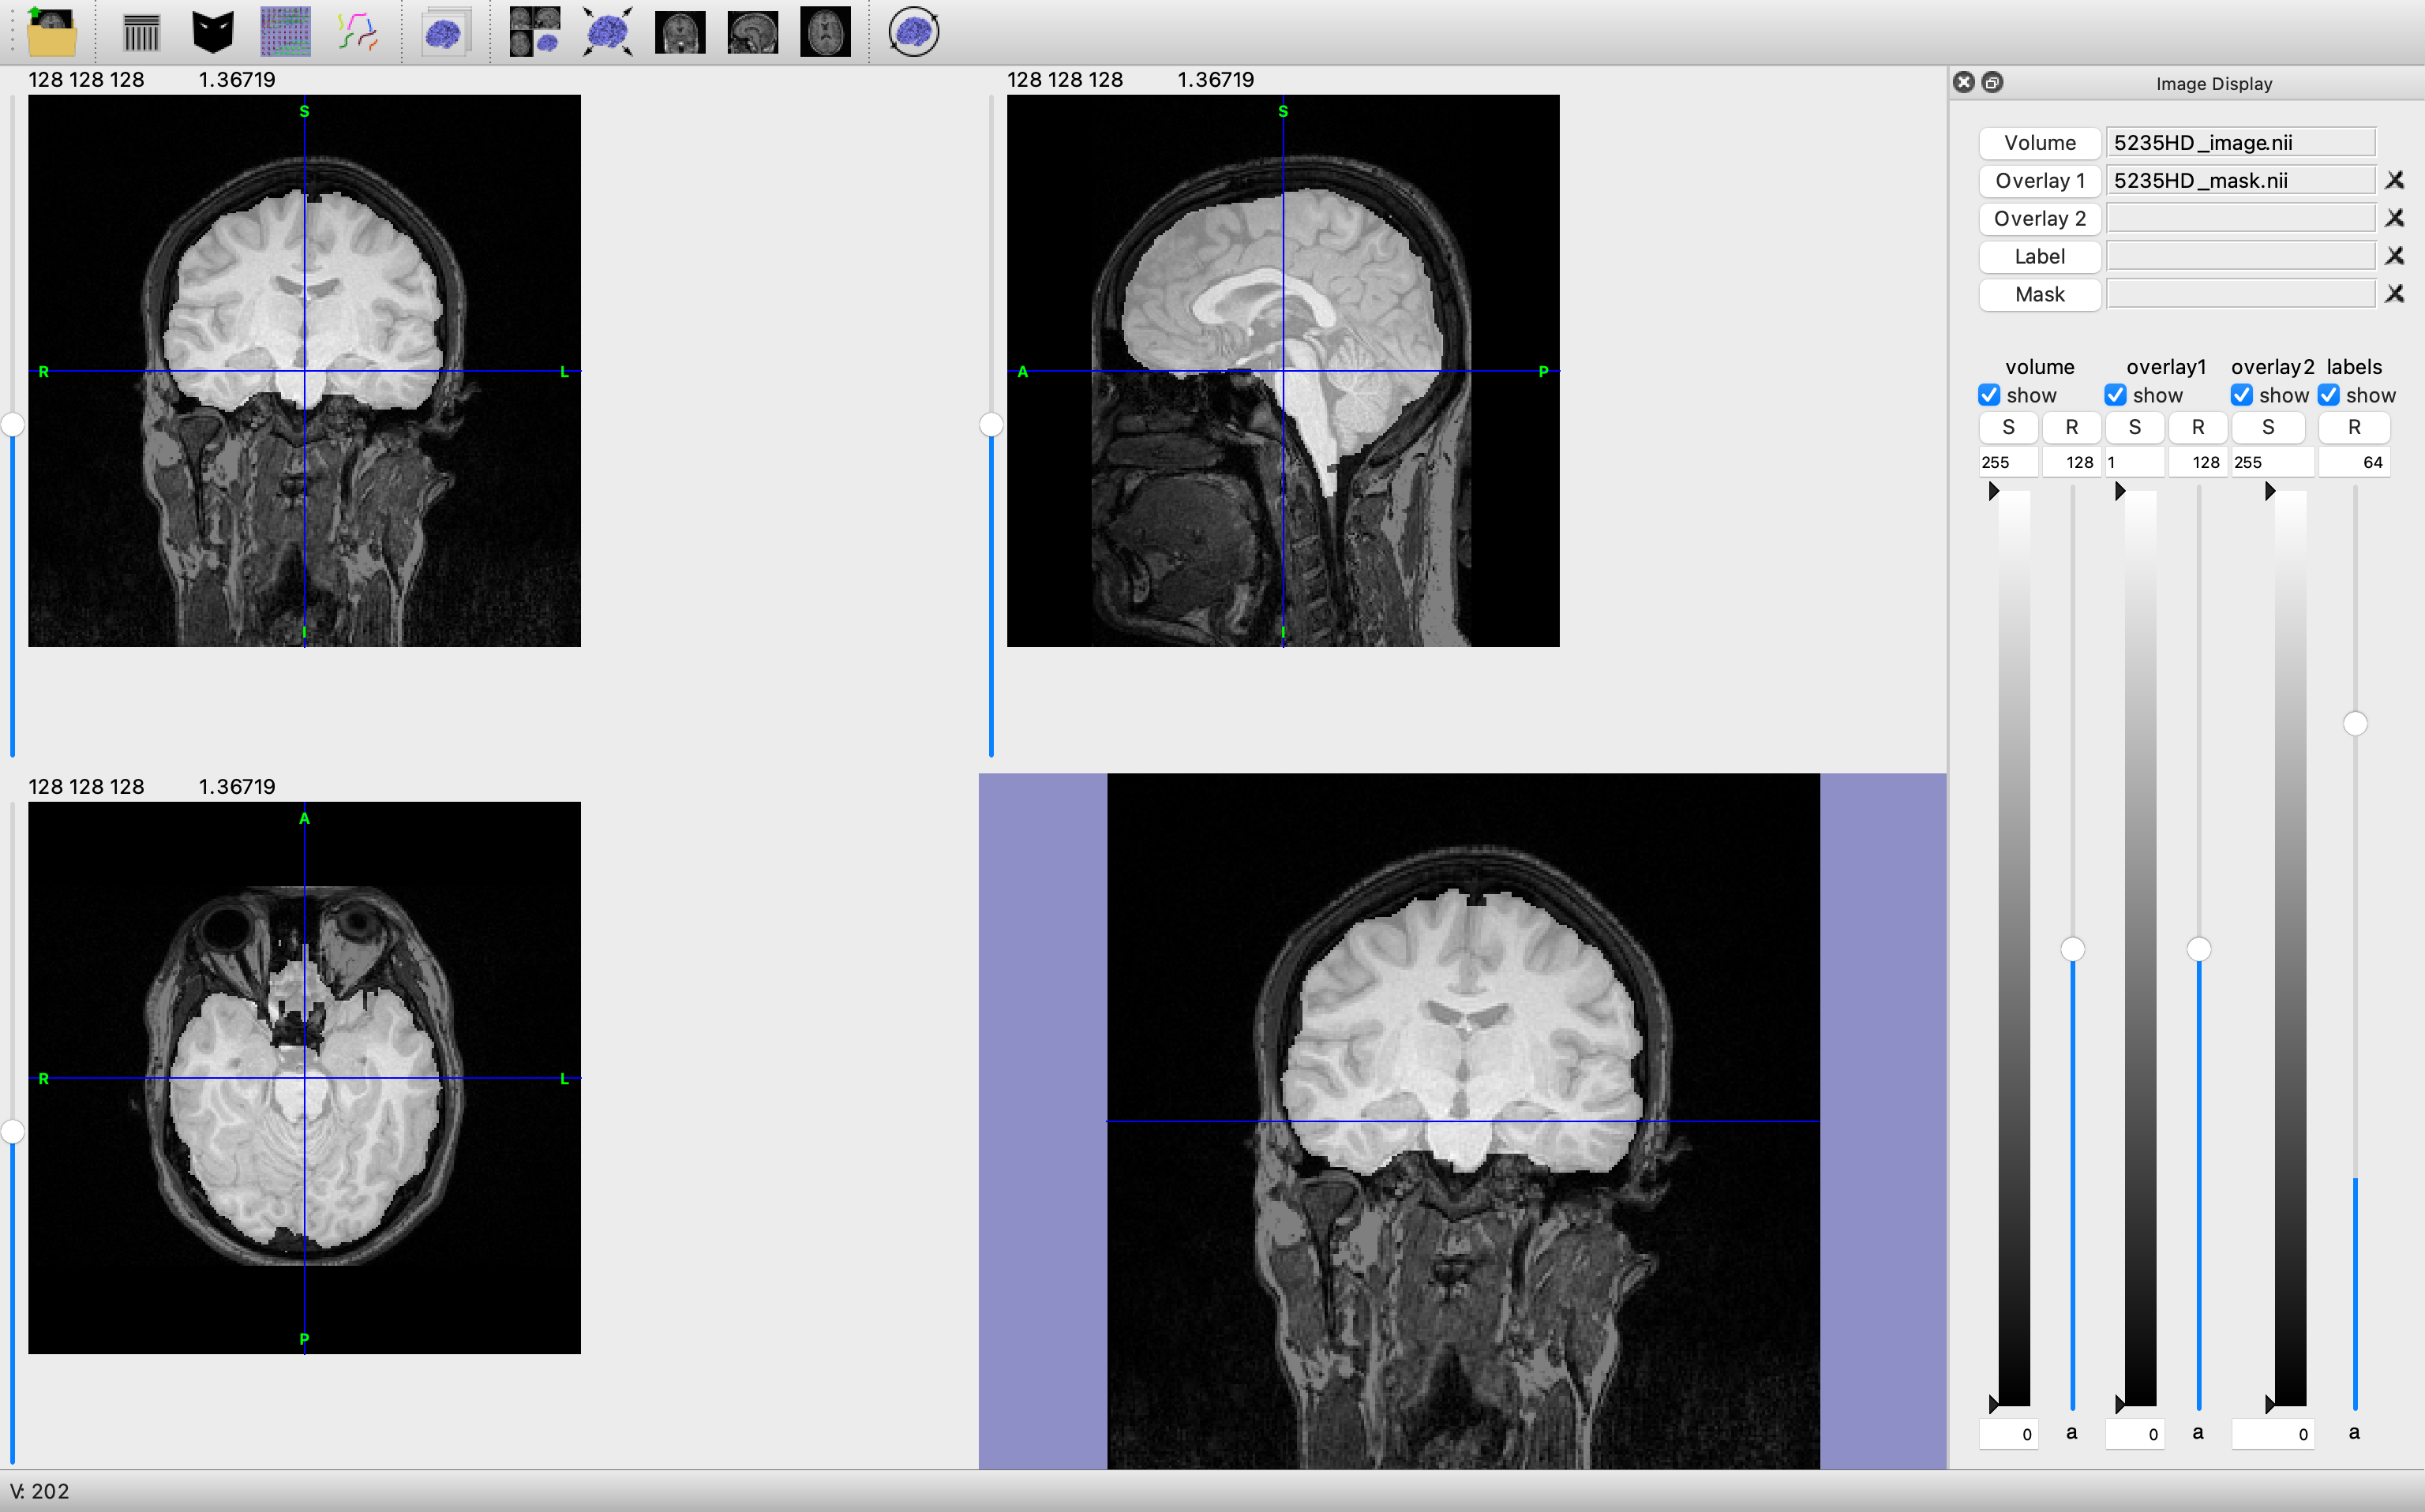
\includegraphics[width=0.67\textwidth]{1}}
\subfigure{
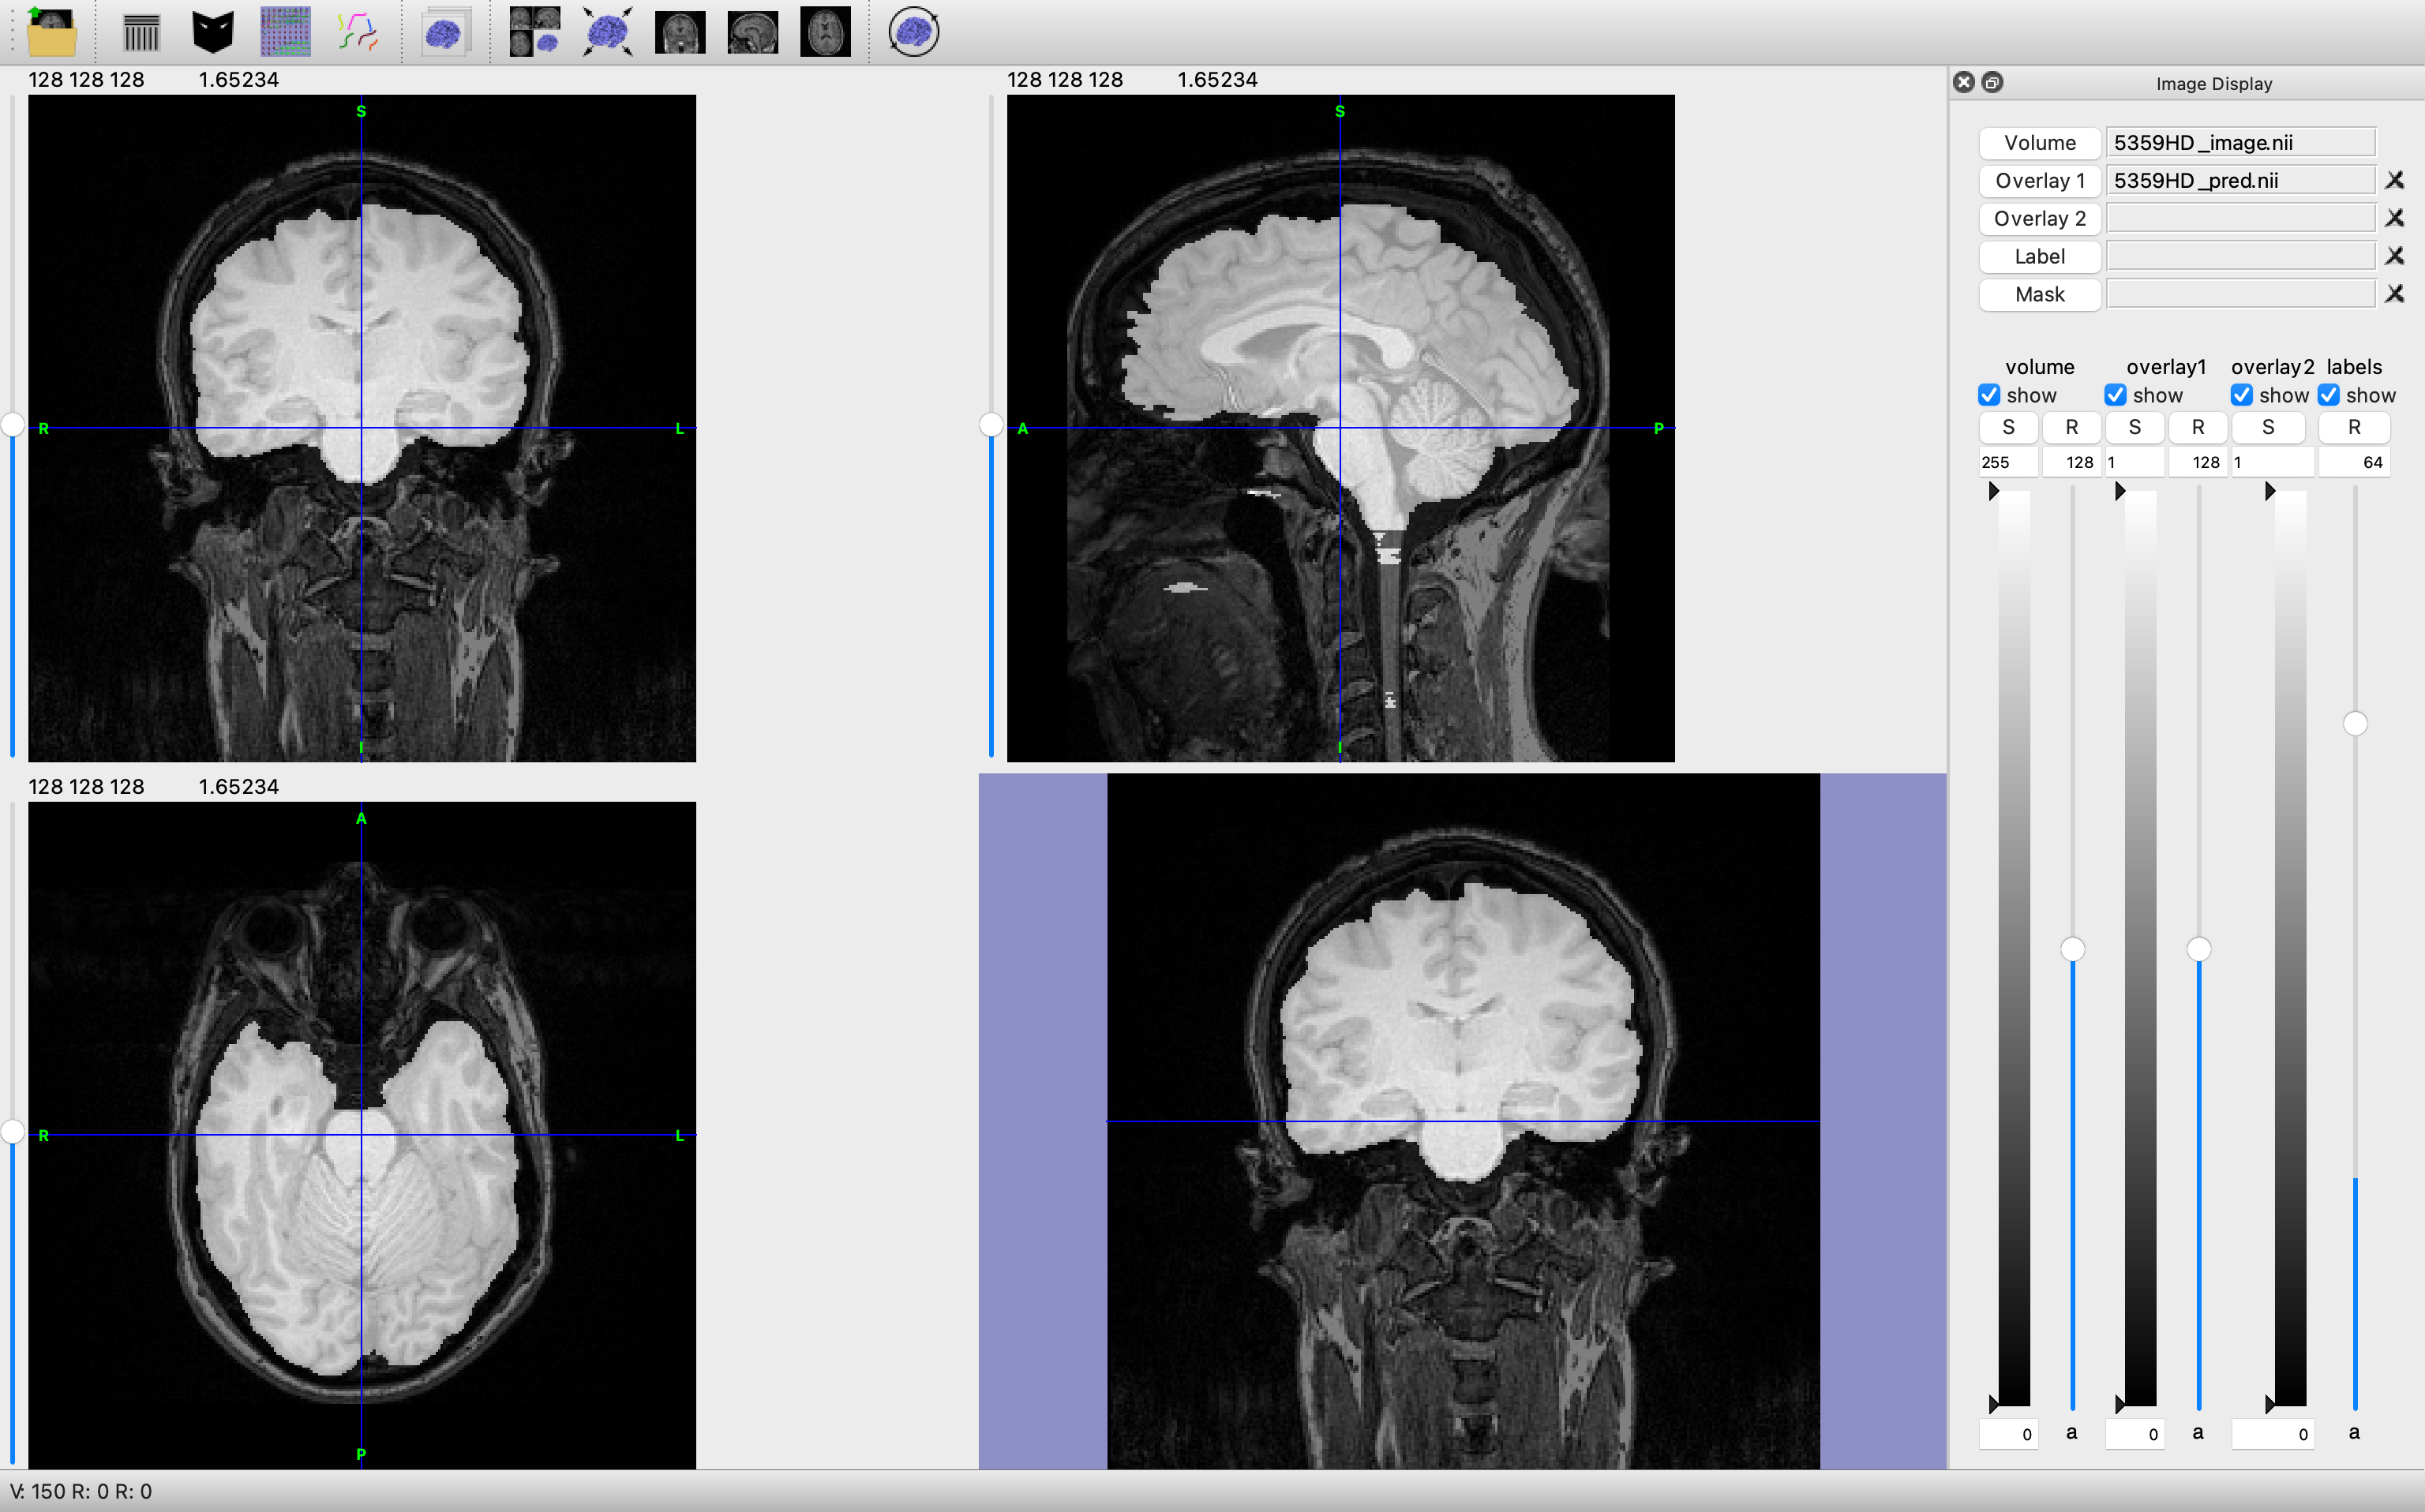
\includegraphics[width=0.67\textwidth]{2}}
\subfigure{
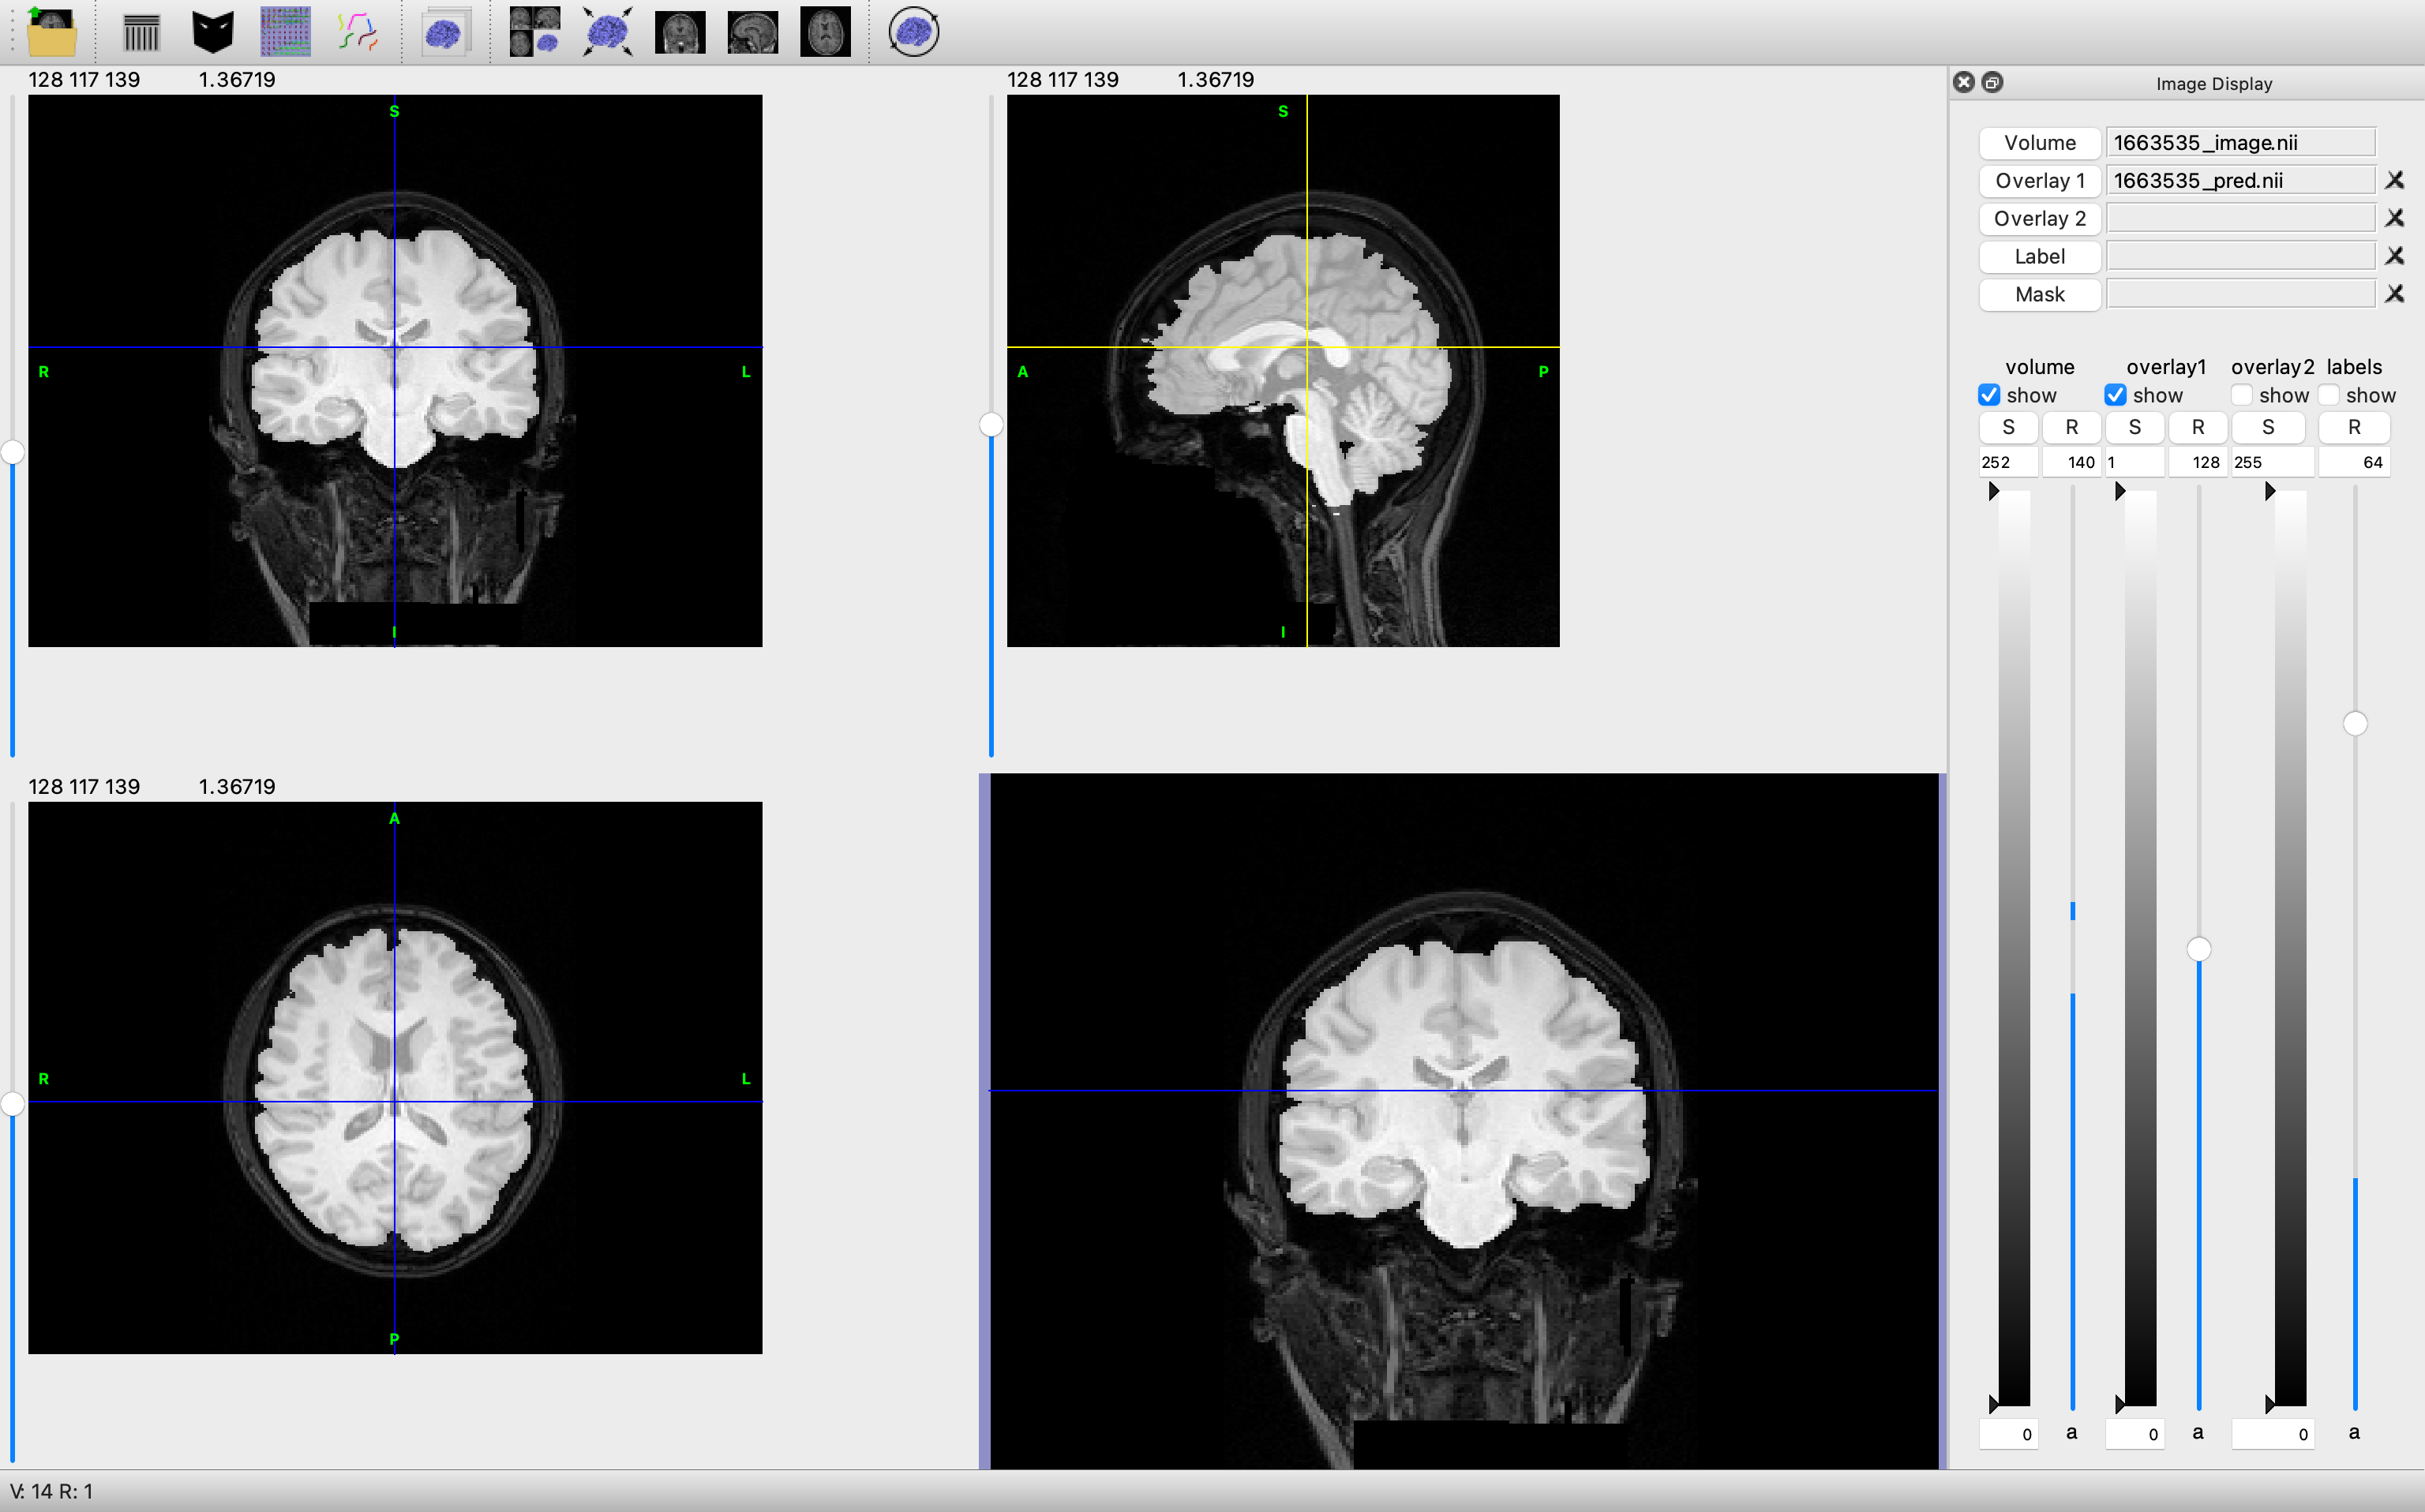
\includegraphics[width=0.67\textwidth]{3}}
\caption{Examples of segmentation}
\end{figure}
\subsection{Postprocessing}
After predicting by the trained model, we got the prediction information in the 'mat' format. Then, we added these slices and predicted masks up respectively and convert them back to '.nii.gz' file.

\section{Results}
To quantify the performance, we utilized Dice metrics to evaluate the accuracy of the segmentation. Figure 2 shows the quantitative comparison of the deep learning model with the algorithm used in the Brainsuite on 18 subjects. The algorithm of the Brainsuite performs better in Dice(0.955) than the deep learning model(0.921).
\begin{figure}[H] 
\centering 
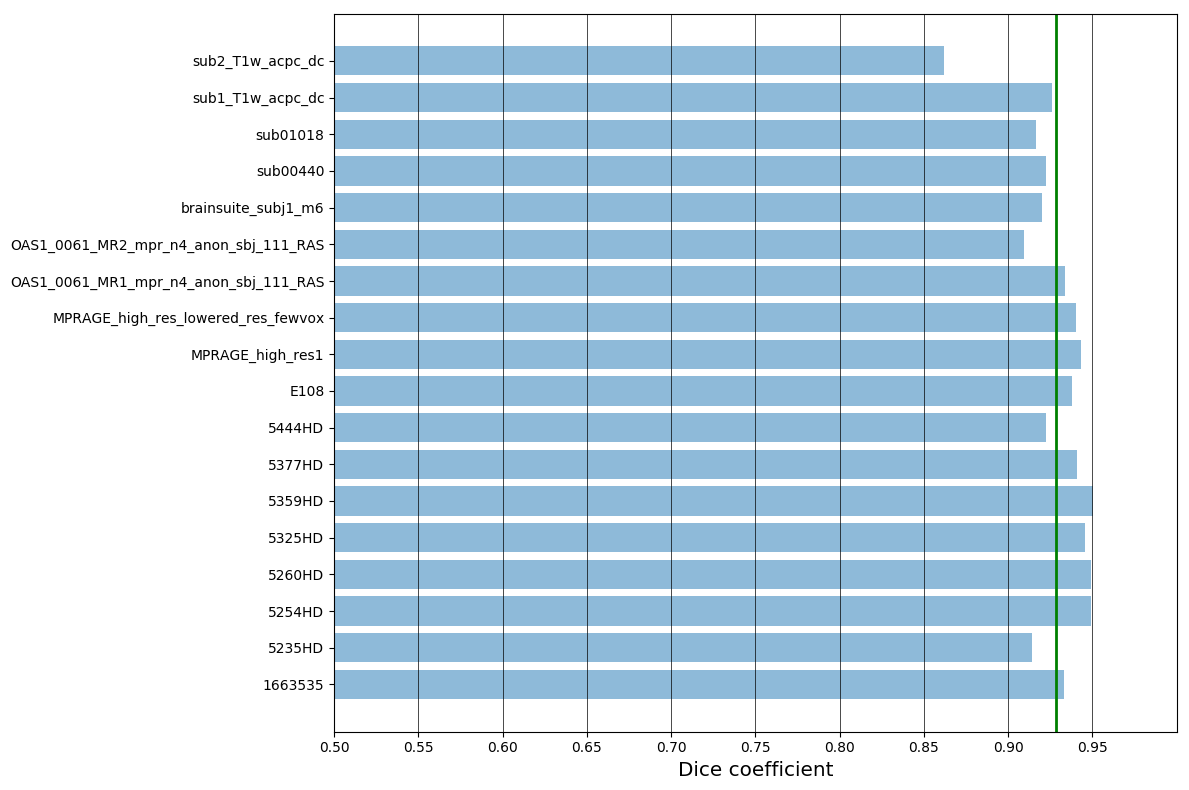
\includegraphics[width=1\textwidth]{DSC} 
\caption{Quantitative analysis of 2 methods} 
\label{DSC} 
\end{figure}

\section{Conclusion}
In conclusion, we replicated this deep learning model and make it easier to execute even the image data are in significantly various sizes, apart from that, we also converted the prediction results into the common format, which is convenient for researchers to analyse.


\bibliography{reference}
\bibliographystyle{plain}

\end{document}